\chapter{Nulla-ismeretű protokoll}

A nulla-ismeretű protokollok a kihívás-válasz protokollokkal szemben képesek úgy bizonyítani a titok ismeretét, hogy nem adnak semmilyen információt a róla. Hogy lássuk hogyan is működik, a formális definíció előtt egy egyszerű példával szeretném szemléltetni cite1,2.

A \ref{Figure::ZKcave} ábrán látható egy barlang. A \textit{C} és \textit{D} pontok között található egy ajtó, amely egy jelszóval nyílik. Ehhez az ajtóhoz csak Aladár tudja a jelszót, senki más. Aladár be szeretné bizonyítani Krisztának, hogy tudja a jelszót, de ezt a jelszó megosztása nélkül szeretné megtenni. A következő a menete Aladár bizonyításának.

\begin{enumerate}
    \item Kriszta megáll az \textit{A} pontnál.
    \item Aladár elsétál a barlangban egészen a \textit{C} vagy \textit{D} pontig.
    \item Ezt követően Kriszta elsétál a \textit{B} pontig, így ő nem tudja, hogy Aladár melyik irányba ment.
    \item Kriszta kiált Aladárnak, hogy:
        \begin{itemize}
            \item a bal útvonalról érkezzen.
            \item a jobb útvonalról érkezzen.
        \end{itemize}
    \item Aladár kinyitja az ajtót, ha szükséges és a kívánt irányból érkezik Krisztához.
    \item Aladár és Kriszta annyiszor ismétlik a lépéseket az 1. lépéstől az 2. lépésig ahányszor szükséges a bizonyításhoz.
\end{enumerate}

\begin{figure}[H]
    \centering
    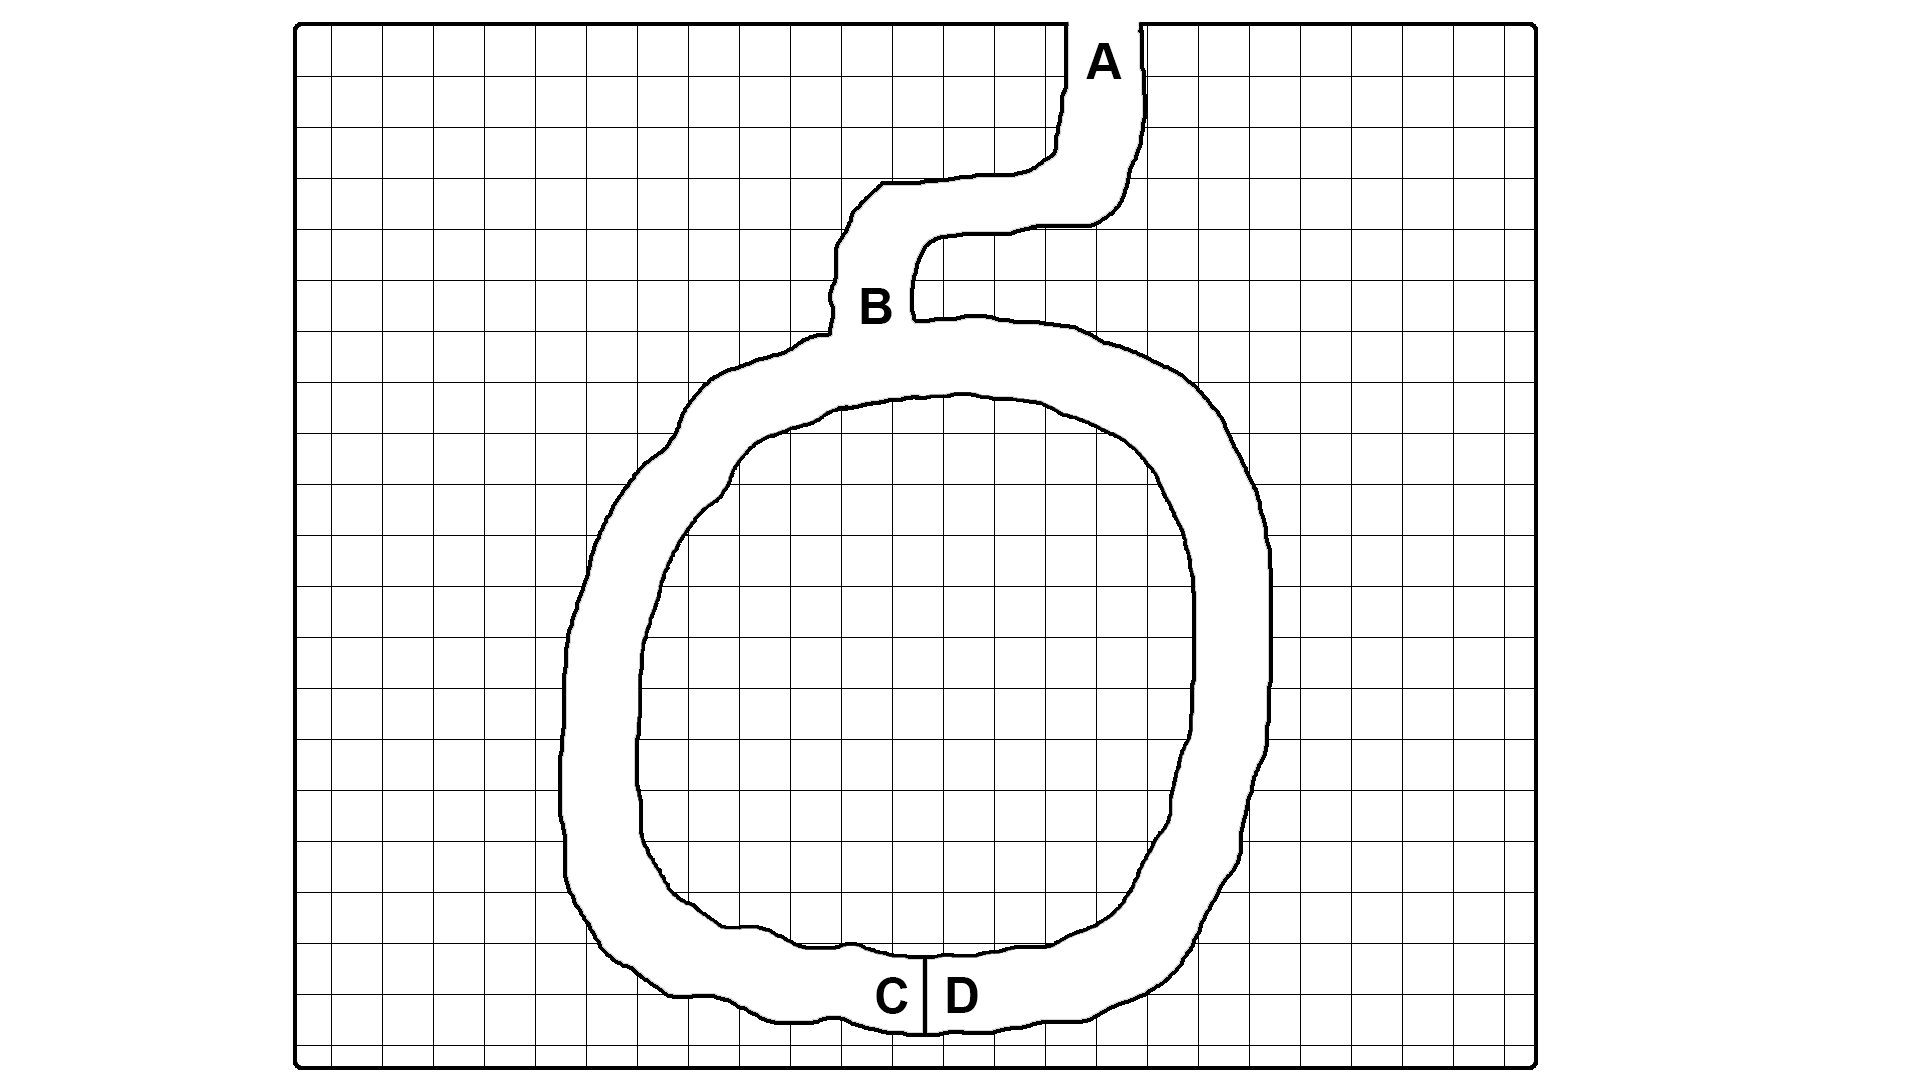
\includegraphics[width=0.6\textwidth]{ZKP.png}
    \caption{A nulla-ismeretű barlang.}
    \label{Figure::ZKcave}
\end{figure}

A többszöri ismétlésre azért van szükség, mert lehet Aladár be szeretné csapni Krisztát, amire minden iterációban 50\% esélye van. Ha abba az irányba ment amelyet Kriszta kiált, akkor szerencsésen be tudta őt csapni, azonban megfelelő ismétlésszámmal sokkal kevesebb esélye van Aladárnak.

A példa egy másik fontos jellemzője az, hogy Aladár ezzel bebizonyíthatta Krisztának, hogy tudja a jelszót, azonban Kriszta nem tud meggyőzni más arról, hogy Aladár tudja a jelszót. Tegyük fel, hogy Kriszta videót készített az egész folyamatról, de így se képes ő maga bizonyítani, hiszen mondhatjuk, hogy a felvétel hamisított, csalás.

Belátható, hogy ez egy nulla ismeretű protokoll, hiszen Kriszta számára bebizonyította Aladár, hogy ismeri a jelszót, méghozzá úgy hogy Kriszta semmit se tudott meg a jelszóról. Emellett Kriszta nem képes bizonyítani harmadik fél számára, hogy Aladár tudja a jelszót.